
\subsubsection{Análisis para $C_{comp}$ en modo tensión, $V_{out} = 10 \si[per-mode=symbol]{\volt}$}




\clearpage

\begin{figure}[H] %htb
\begin{center}
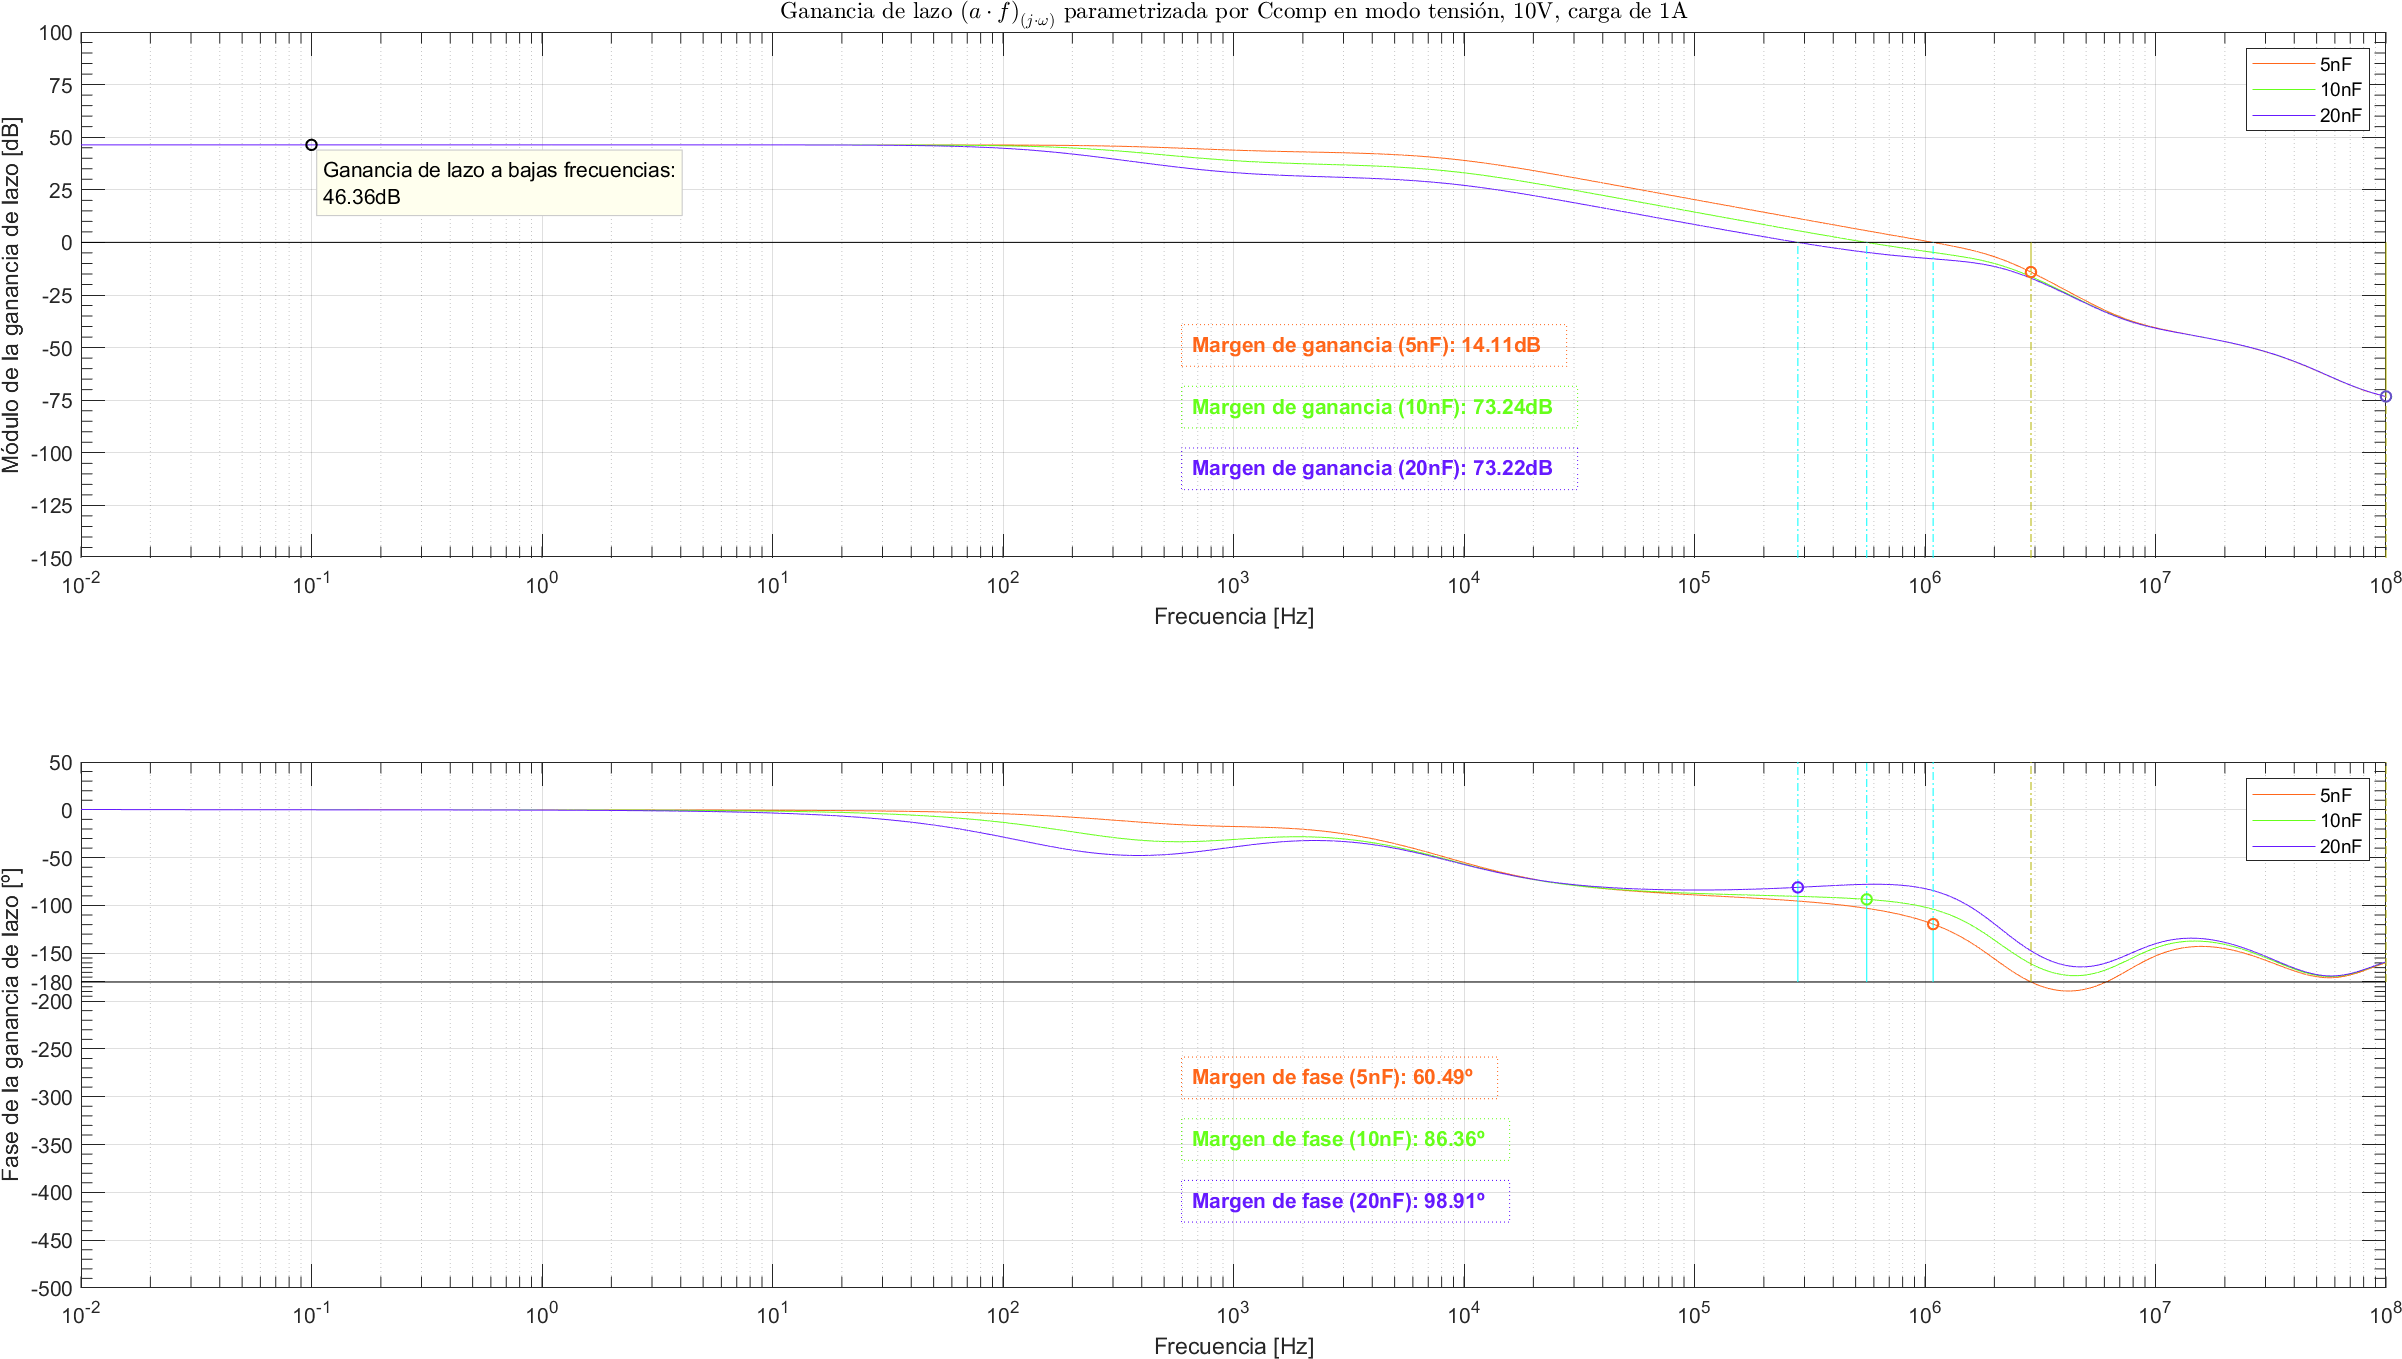
\includegraphics[width=1.1 \textwidth, angle=90]{./img/plots/loop/power_supply_CCOMP_LOOP_Modo1.png}
\caption{\label{fig:fig_power_supply_CCOMP_LOOP_Modo1}\footnotesize{Ganancia de lazo en modo tensión, $V_{out} = 10 \si[per-mode=symbol]{\volt}$, en función de la frecuencia parametrizada por $C_{comp}$.}}
\end{center}
\end{figure}


\clearpage

\begin{figure}[H] %htb
\begin{center}
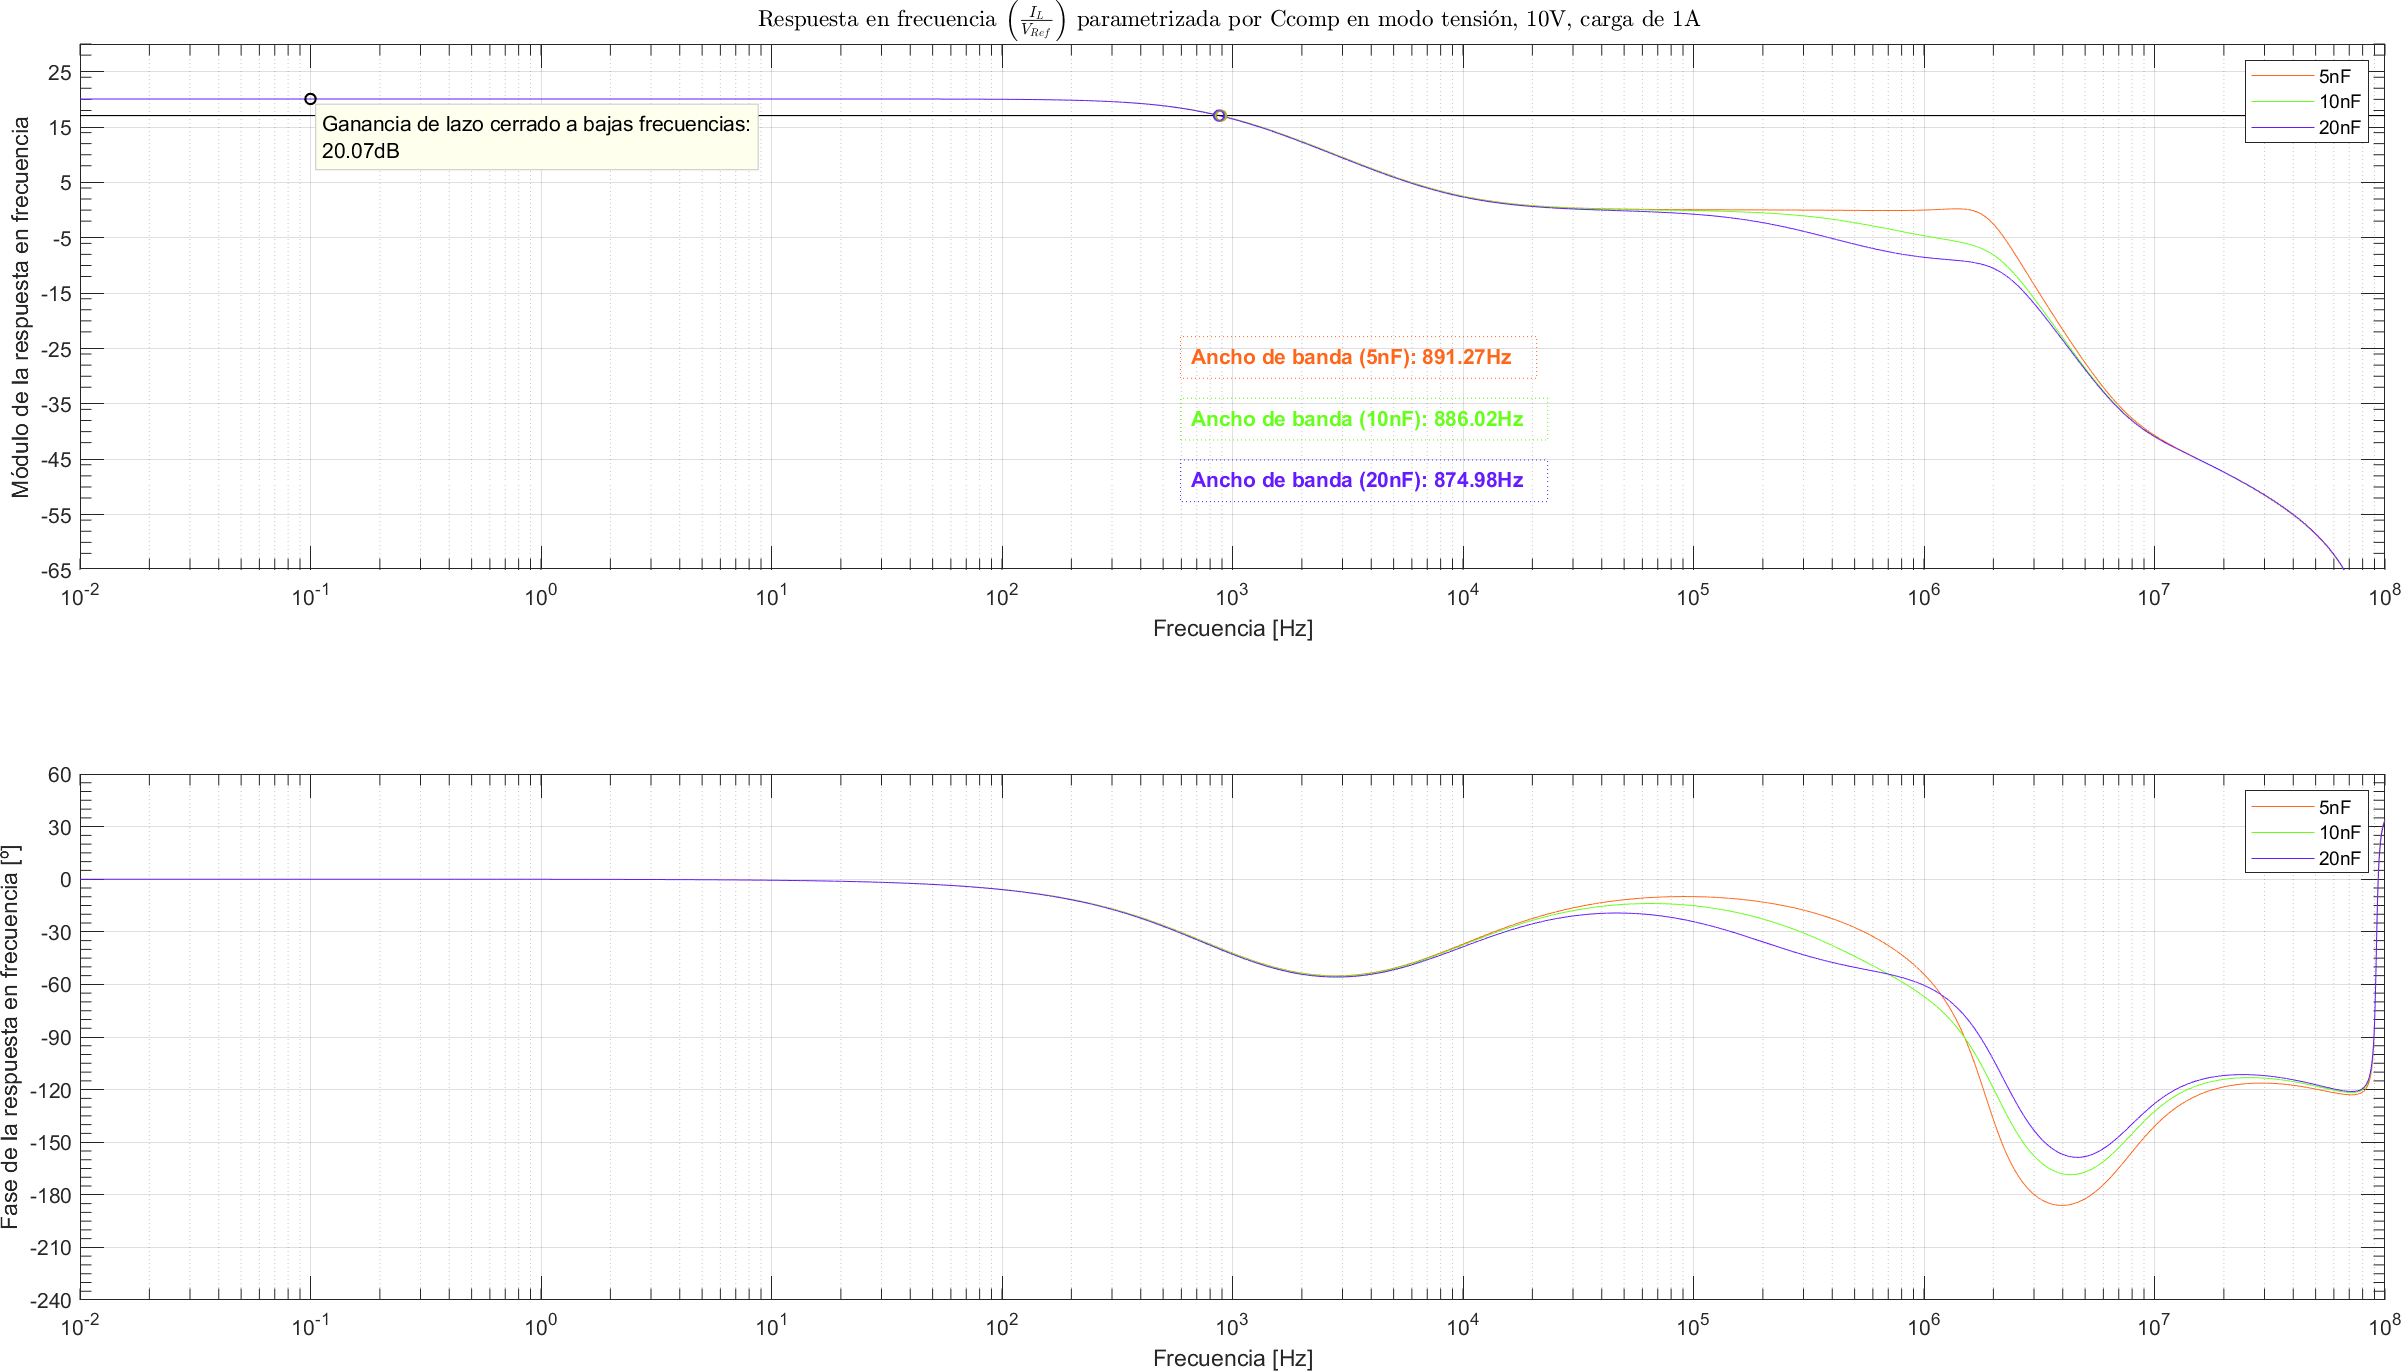
\includegraphics[width=1.1 \textwidth, angle=90]{./img/plots/rf/power_supply_CCOMP_RF_Modo1.png}
\caption{\label{fig:fig_power_supply_CCOMP_RF_Modo1}\footnotesize{Respuesta en frecuencia en modo tensión, $V_{out} = 10 \si[per-mode=symbol]{\volt}$, en función de la frecuencia parametrizada por $C_{comp}$.}}
\end{center}
\end{figure}

\clearpage

\begin{figure}[H] %htb
\begin{center}
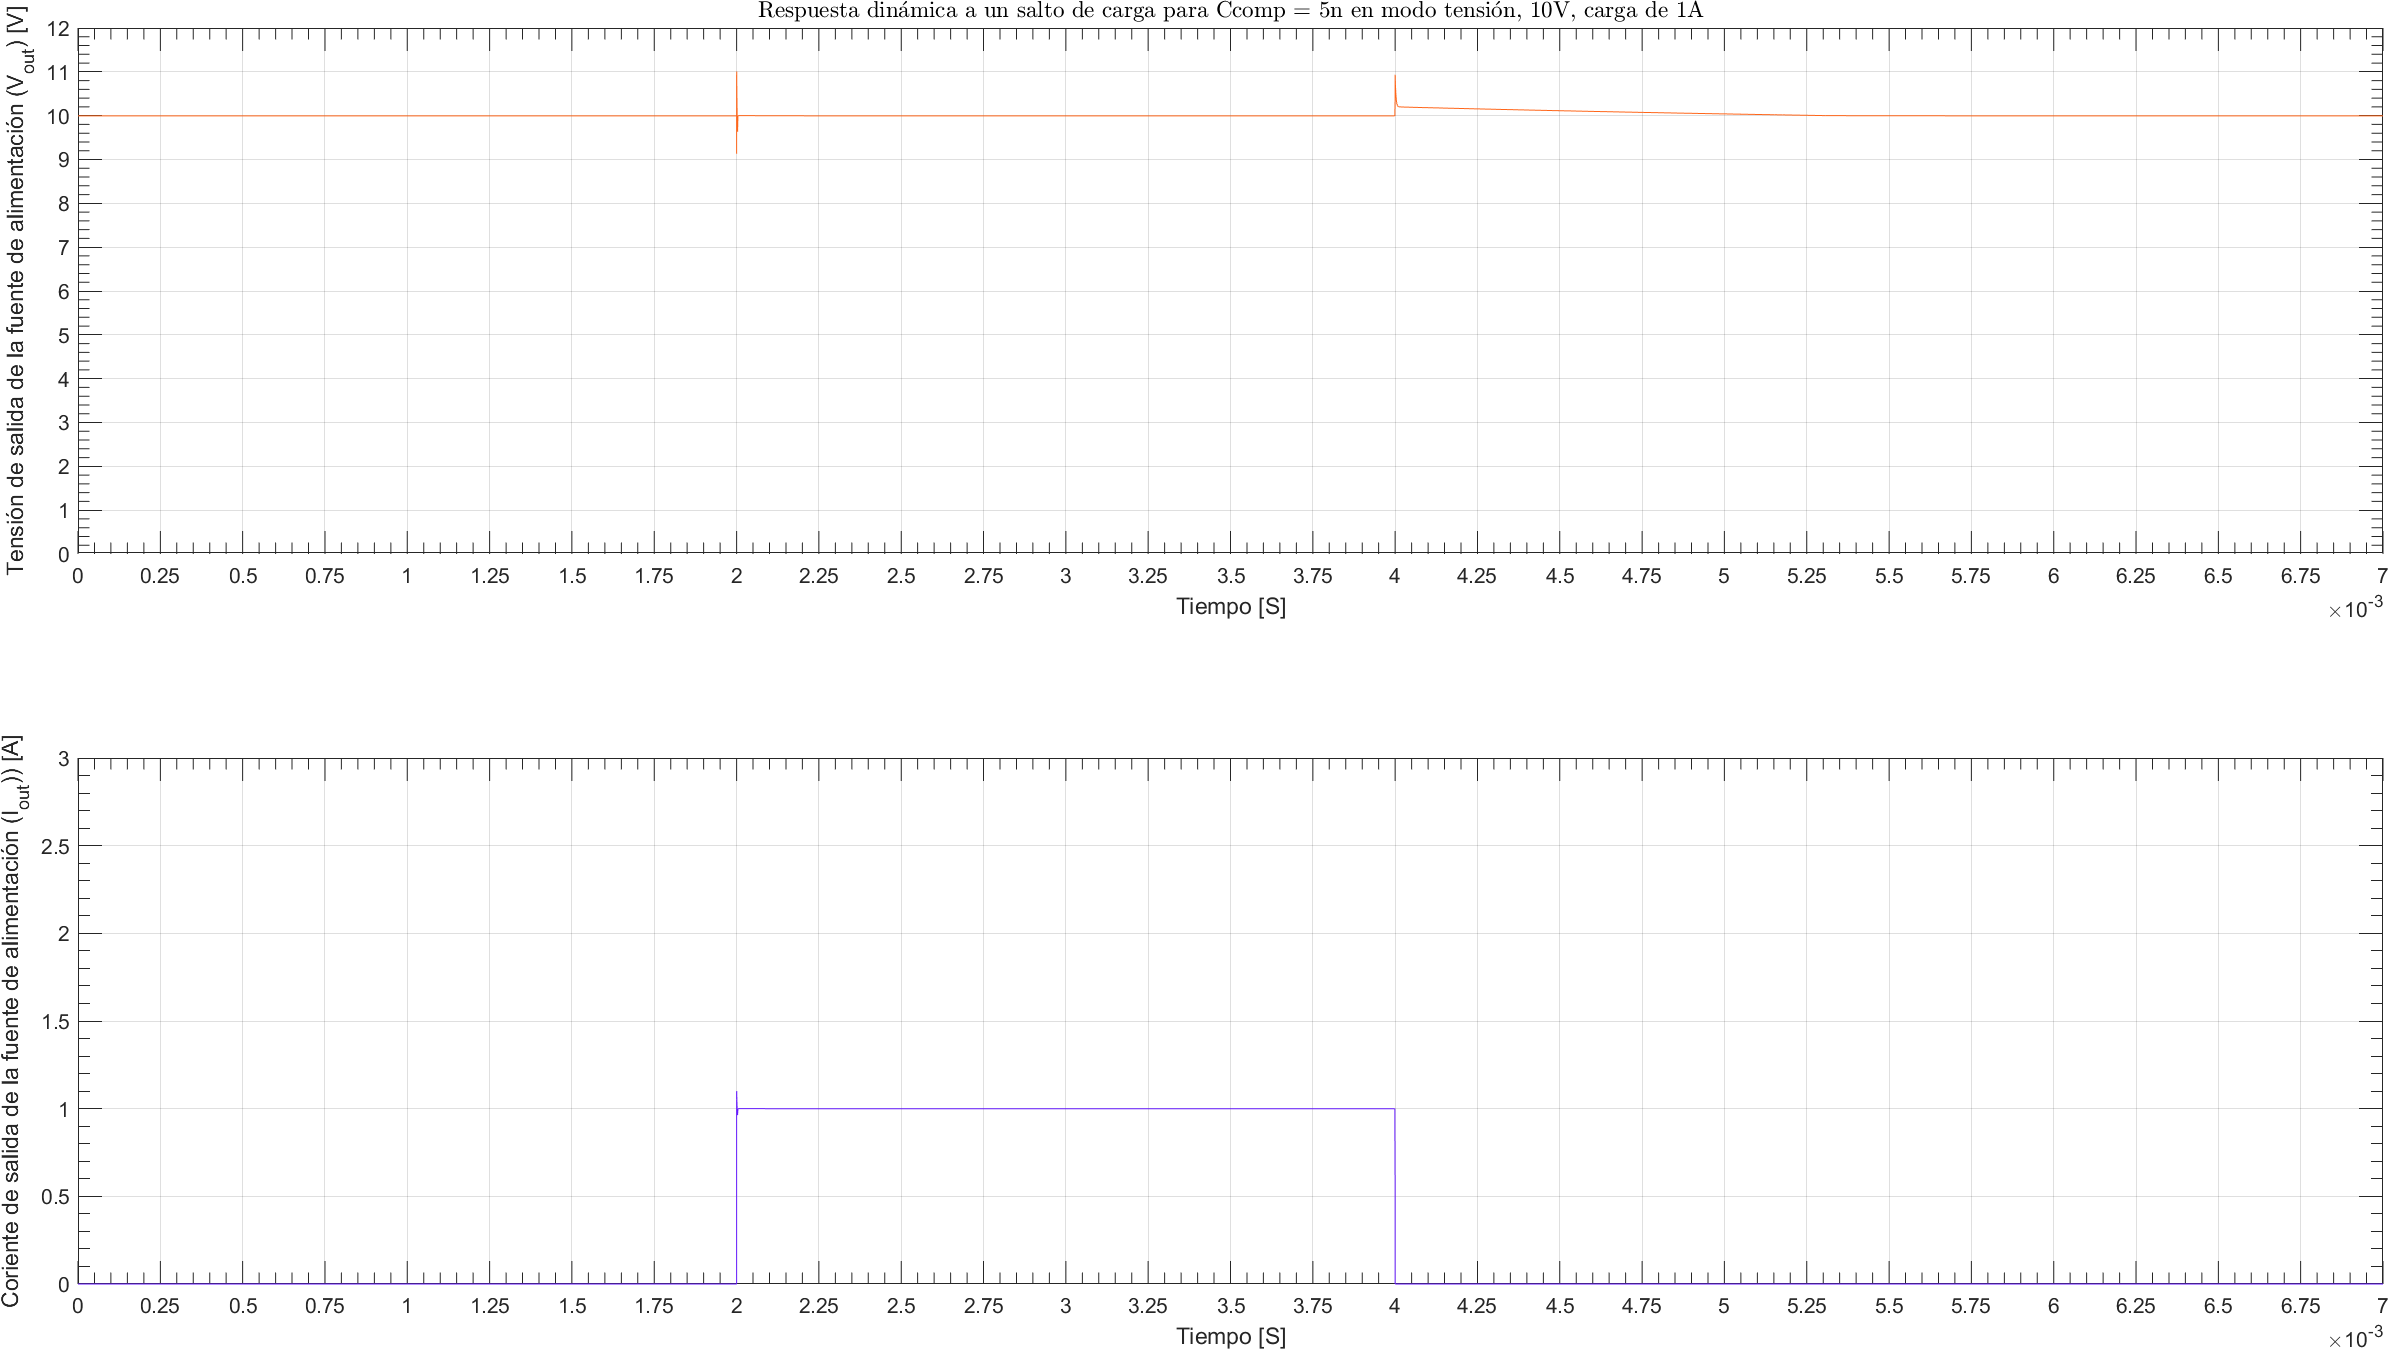
\includegraphics[width=1.1 \textwidth, angle=90]{./img/plots/dynamic/power_supply_CCOMP_5n_STEP_Modo1.png}
\caption{\label{fig:fig_power_supply_CCOMP_STEP_5n_Modo1}\footnotesize{Respuesta dinámica en modo tensión, $V_{out} = 10 \si[per-mode=symbol]{\volt}$, para $C_{comp} = 5 \si[per-mode=symbol]{\nano\farad} $ .}}
\end{center}
\end{figure}

\clearpage

\begin{figure}[H] %htb
\begin{center}
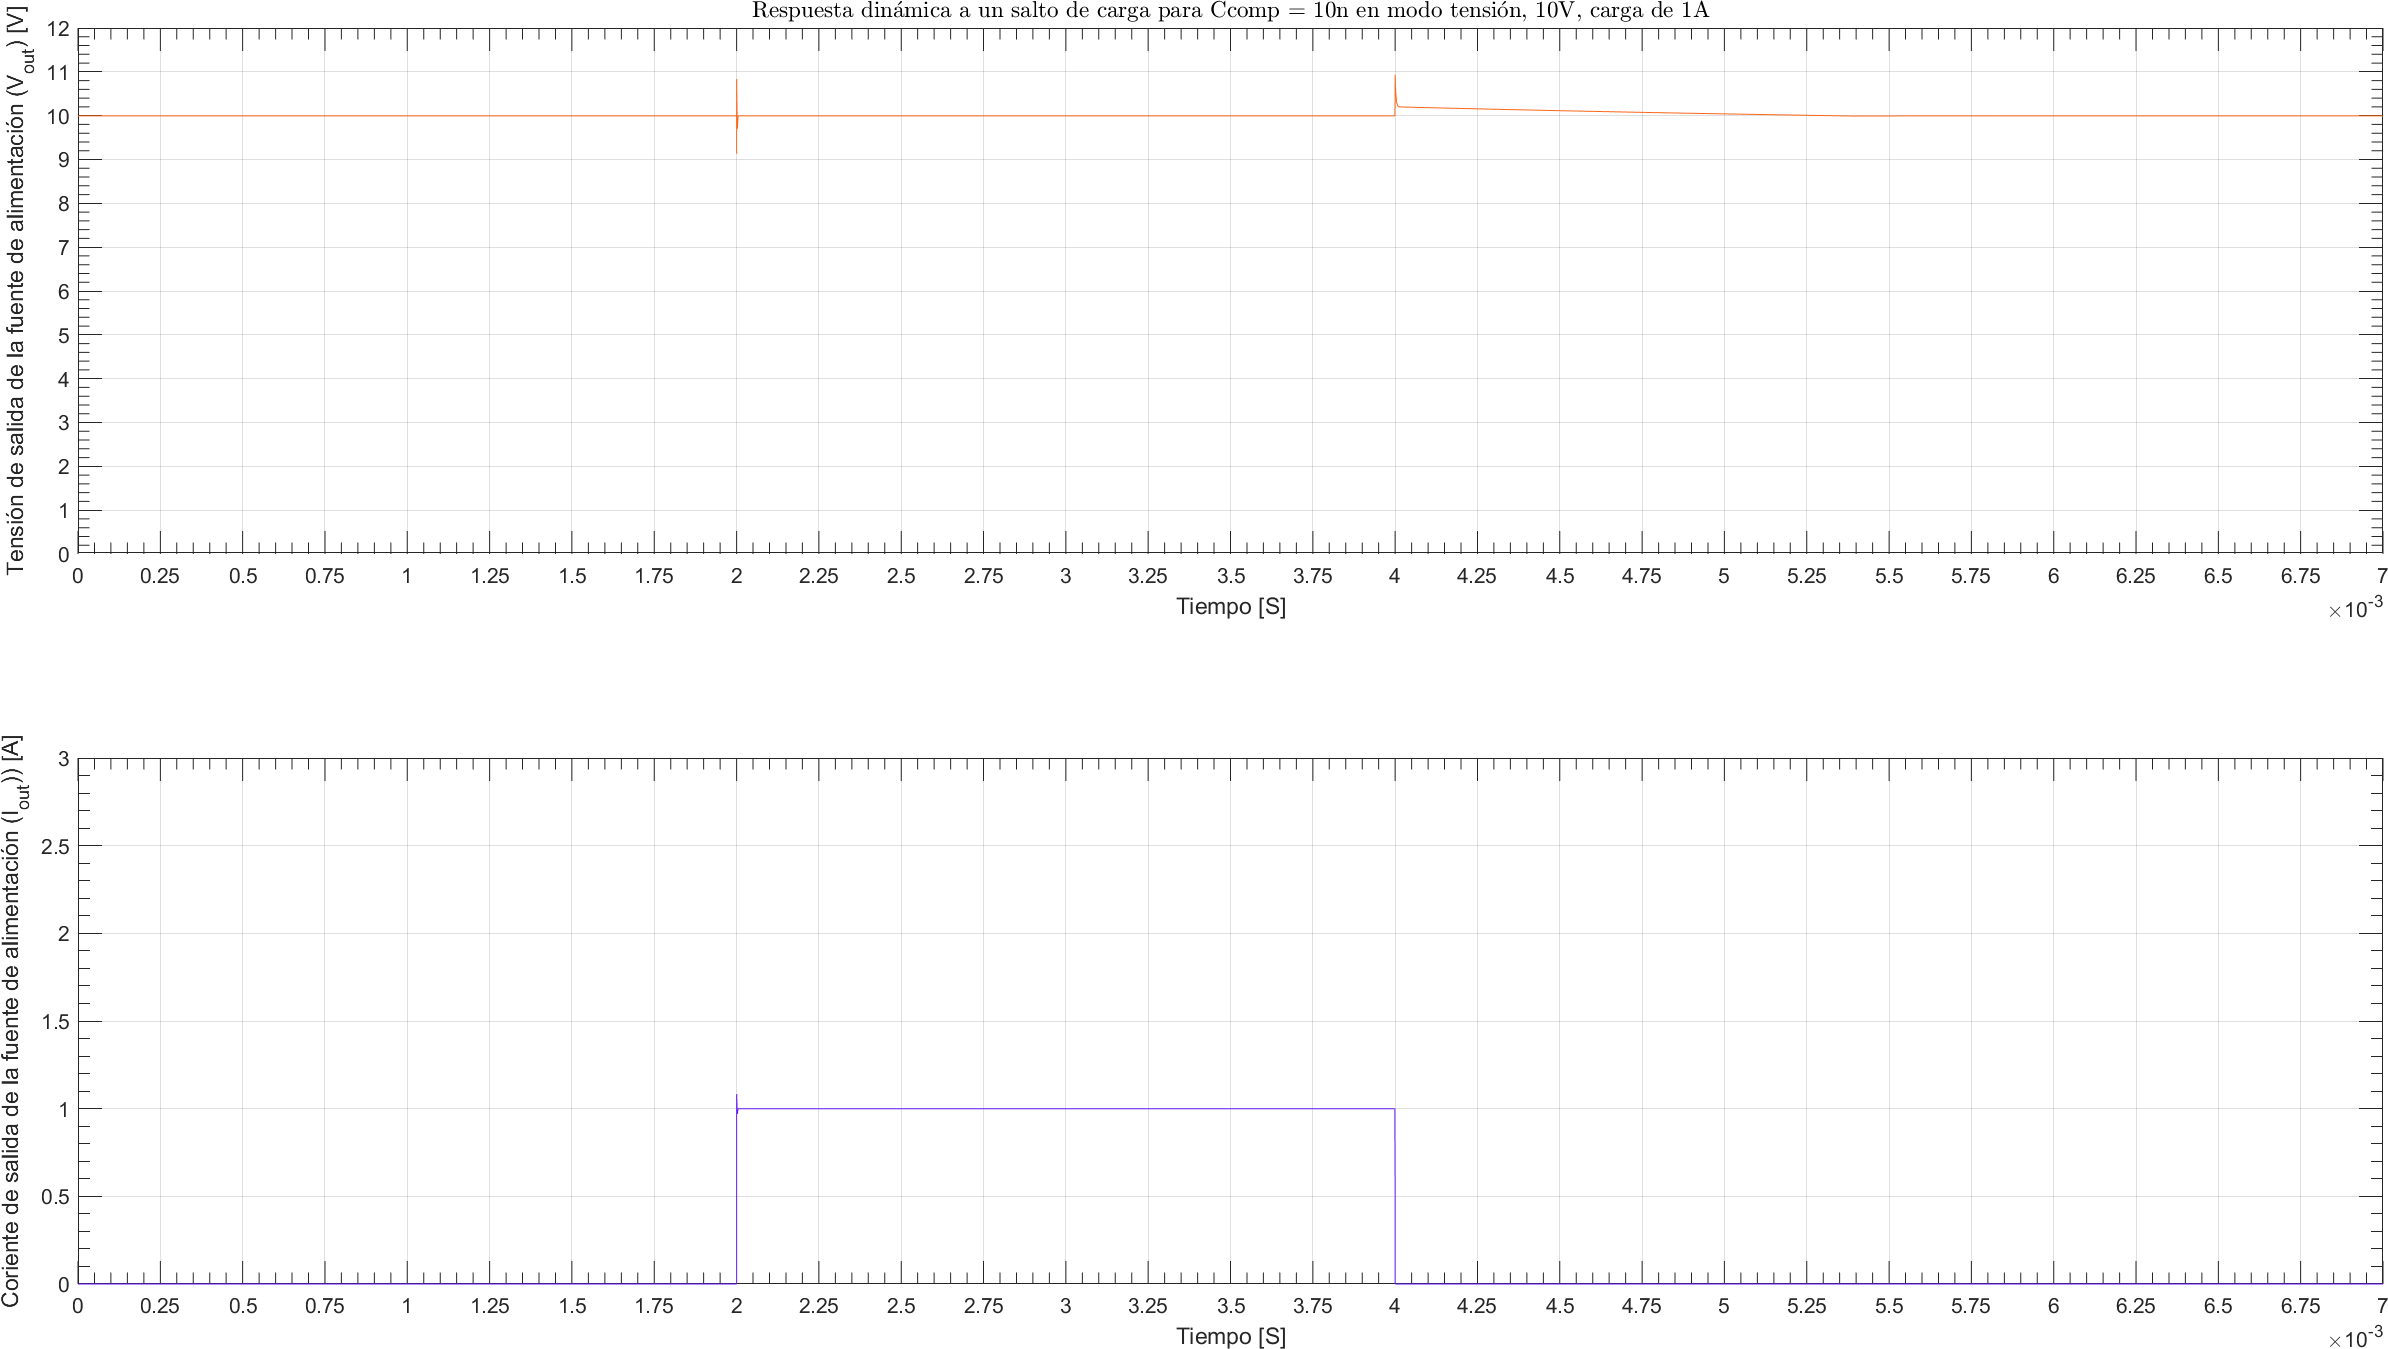
\includegraphics[width=1.1 \textwidth, angle=90]{./img/plots/dynamic/power_supply_CCOMP_10n_STEP_Modo1.png}
\caption{\label{fig:fig_power_supply_CCOMP_STEP_10n_Modo1}\footnotesize{Respuesta dinámica en modo tensión, $V_{out} = 10 \si[per-mode=symbol]{\volt}$, para $C_{comp} = 10 \si[per-mode=symbol]{\nano\farad} $ .}}
\end{center}
\end{figure}

\clearpage

\begin{figure}[H] %htb
\begin{center}
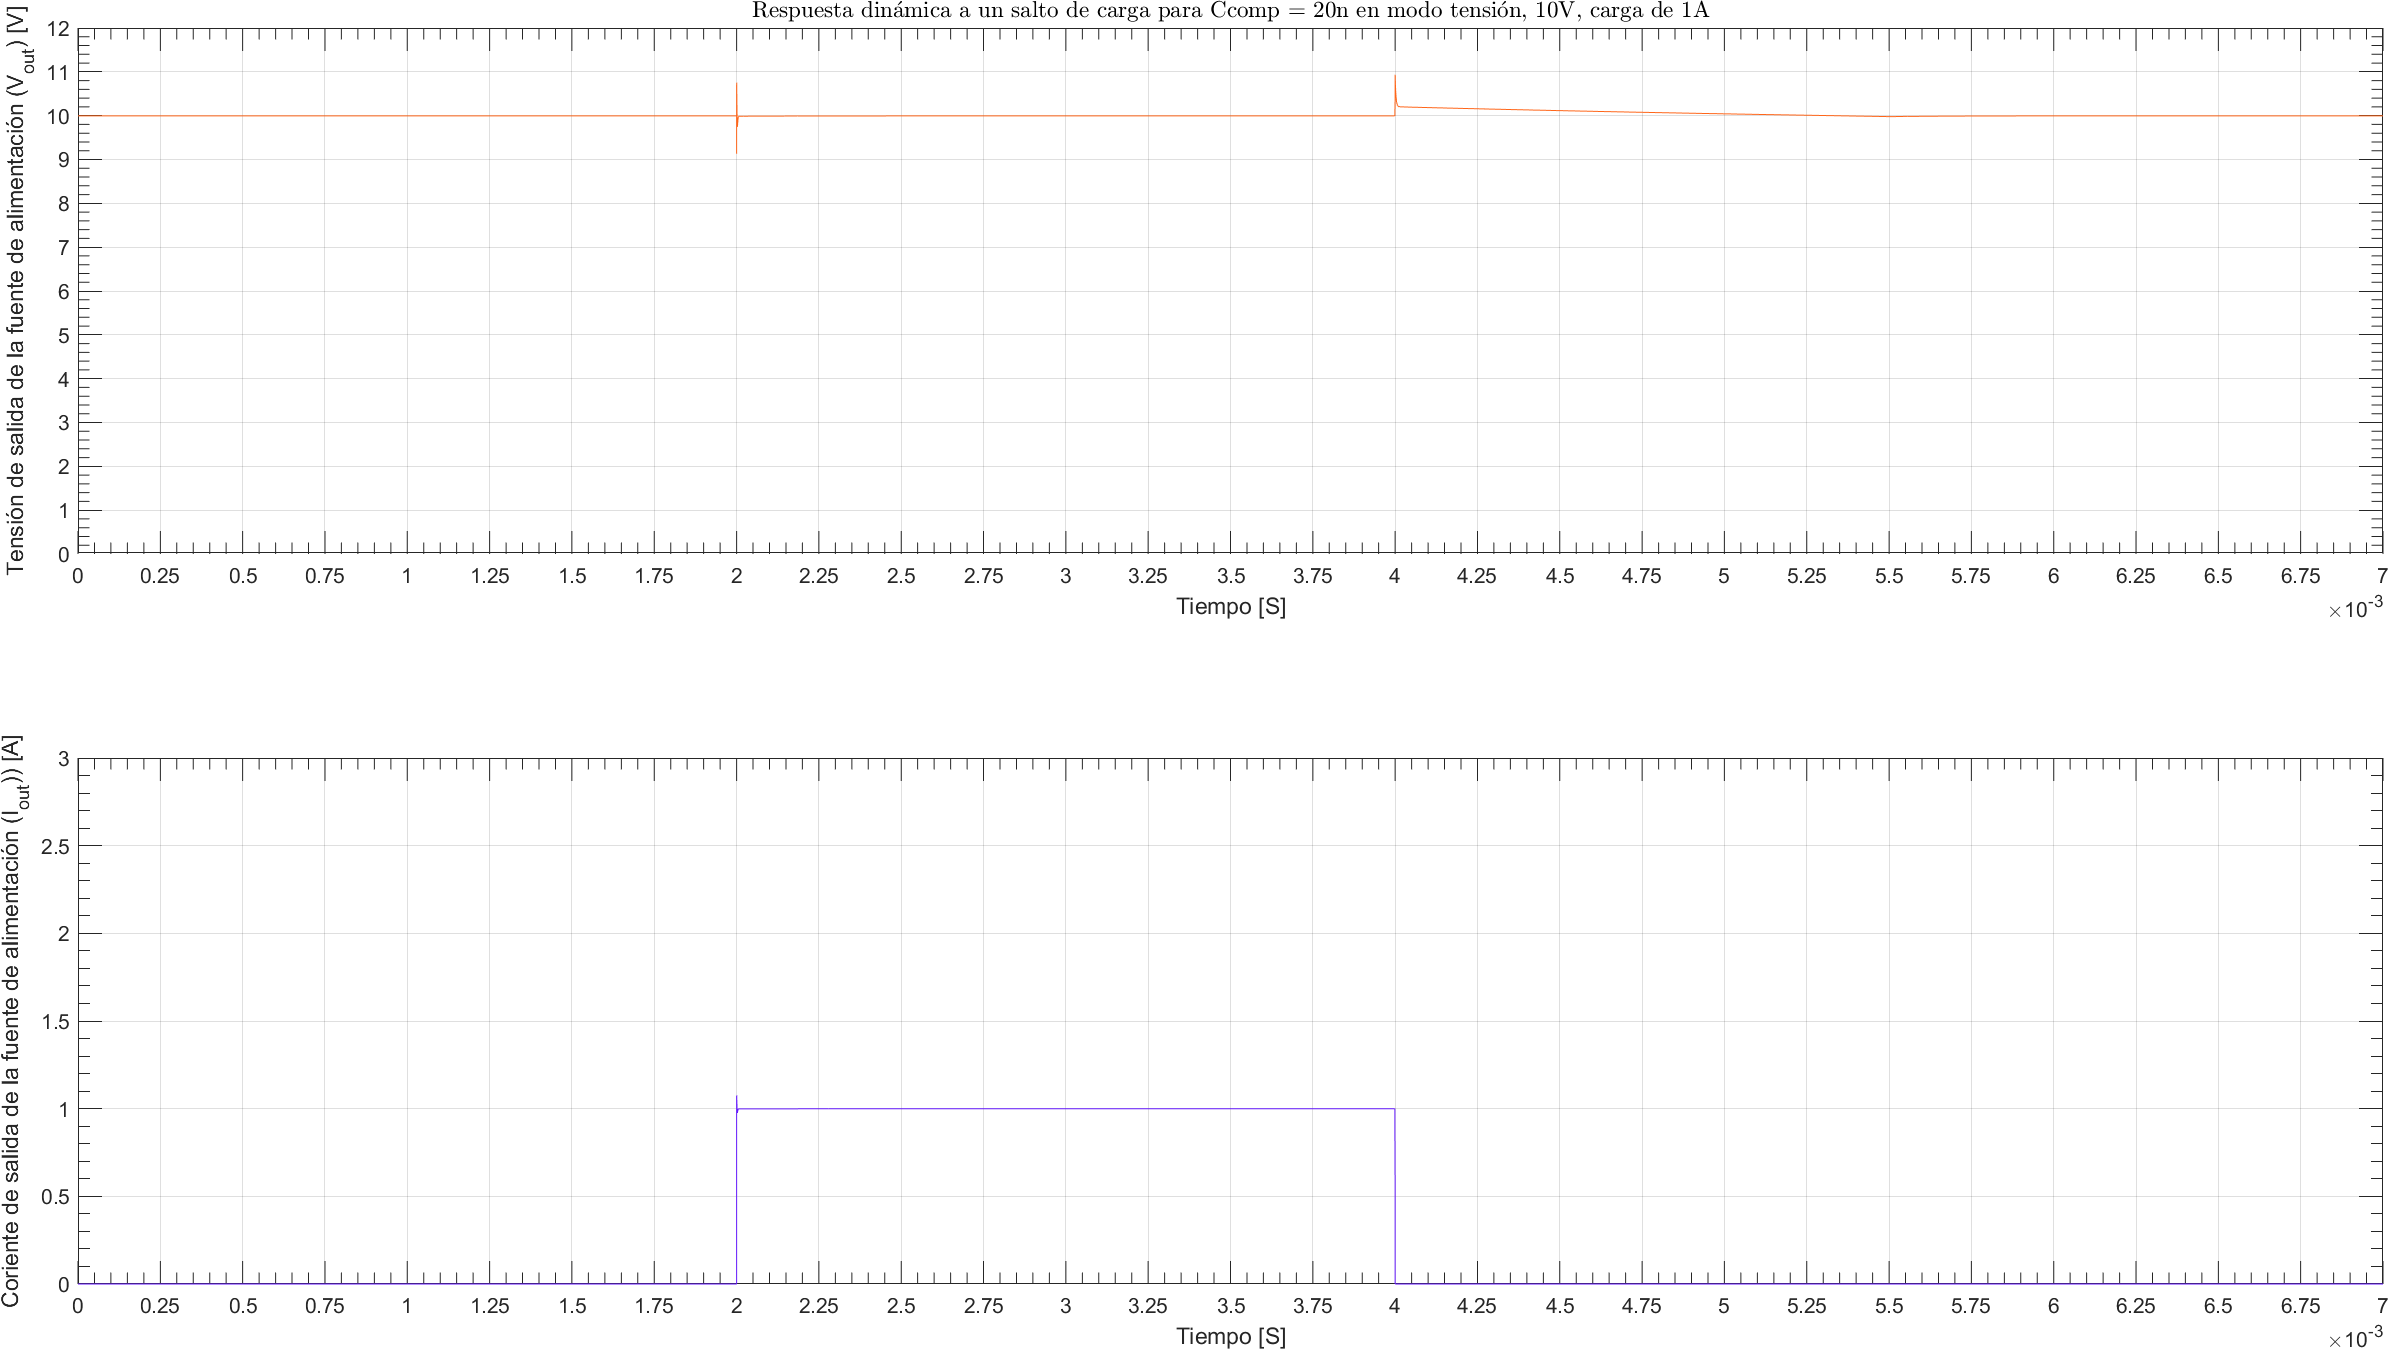
\includegraphics[width=1.1 \textwidth, angle=90]{./img/plots/dynamic/power_supply_CCOMP_20n_STEP_Modo1.png}
\caption{\label{fig:fig_power_supply_CCOMP_STEP_20n_Modo1}\footnotesize{Respuesta dinámica en modo tensión, $V_{out} = 10 \si[per-mode=symbol]{\volt}$, para $C_{comp} = 20 \si[per-mode=symbol]{\nano\farad} $ .}}
\end{center}
\end{figure}

\clearpage














%
%\subsubsection{Análisis para $C_{comp}$ en modo tensión, $V_{out} = 1 \si[per-mode=symbol]{\volt}$}
%
%
%
%\clearpage
%
%\begin{figure}[H] %htb
%\begin{center}
%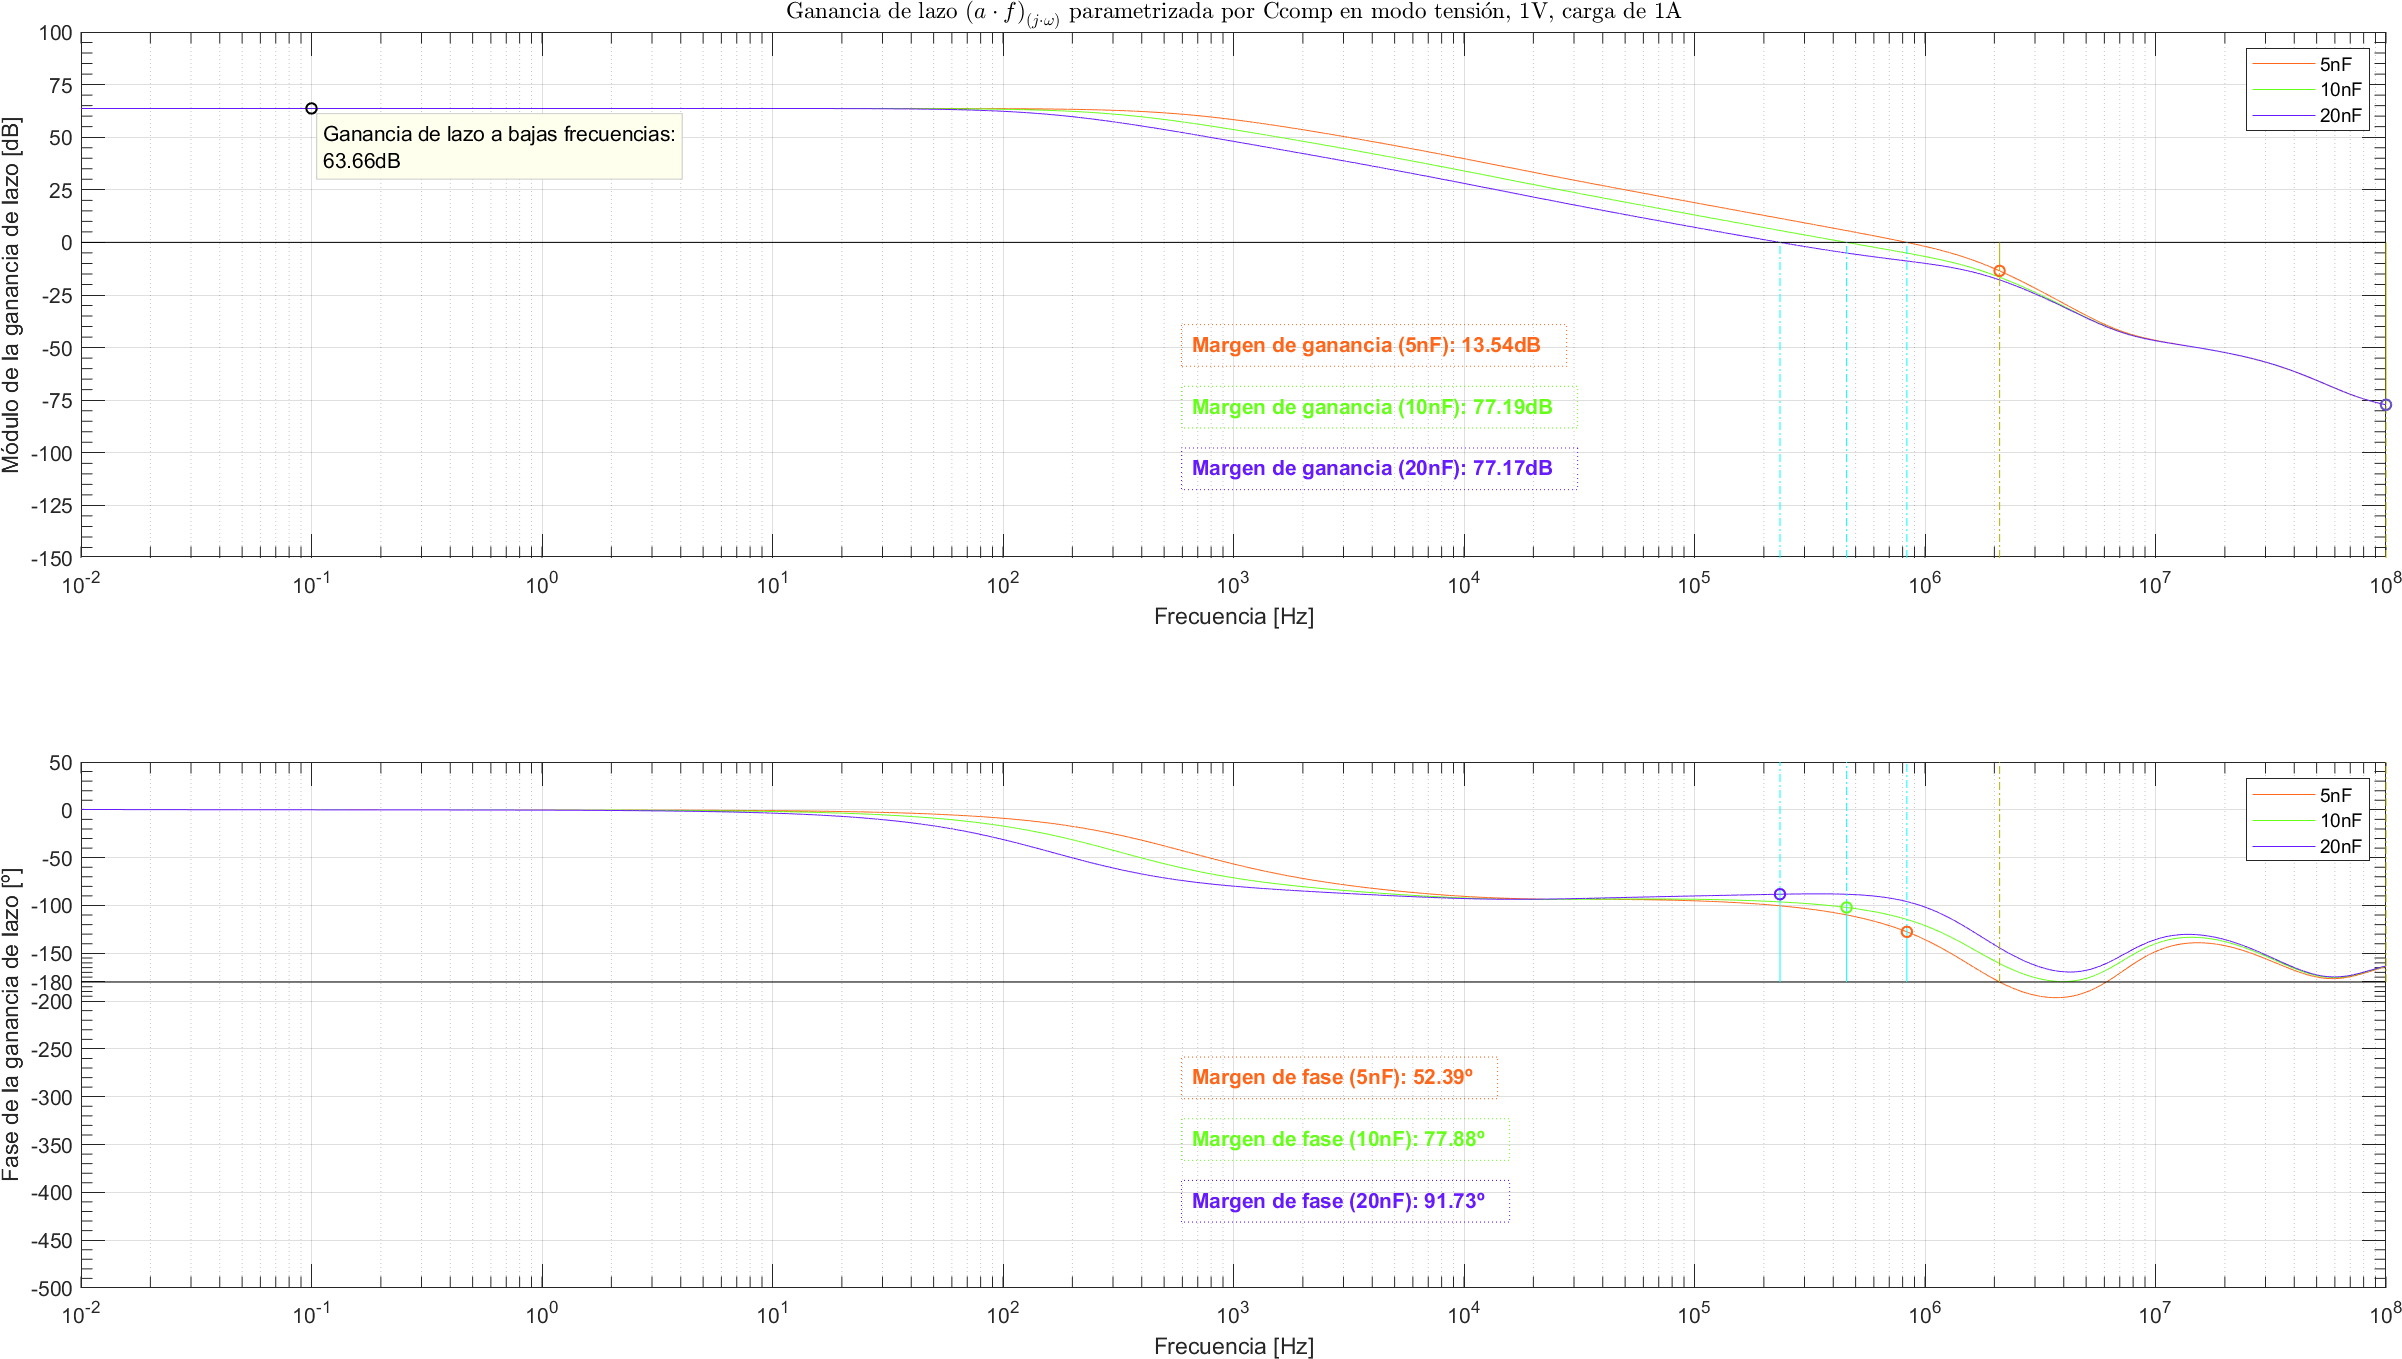
\includegraphics[width=1.1 \textwidth, angle=90]{./img/plots/loop/power_supply_CCOMP_LOOP_Modo2.png}
%\caption{\label{fig:fig_power_supply_CCOMP_LOOP_Modo2}\footnotesize{Ganancia de lazo en modo tensión, $V_{out} = 1 \si[per-mode=symbol]{\volt}$, en función de la frecuencia parametrizada por $C_{comp}$.}}
%\end{center}
%\end{figure}
%
%
%\clearpage
%
%\begin{figure}[H] %htb
%\begin{center}
%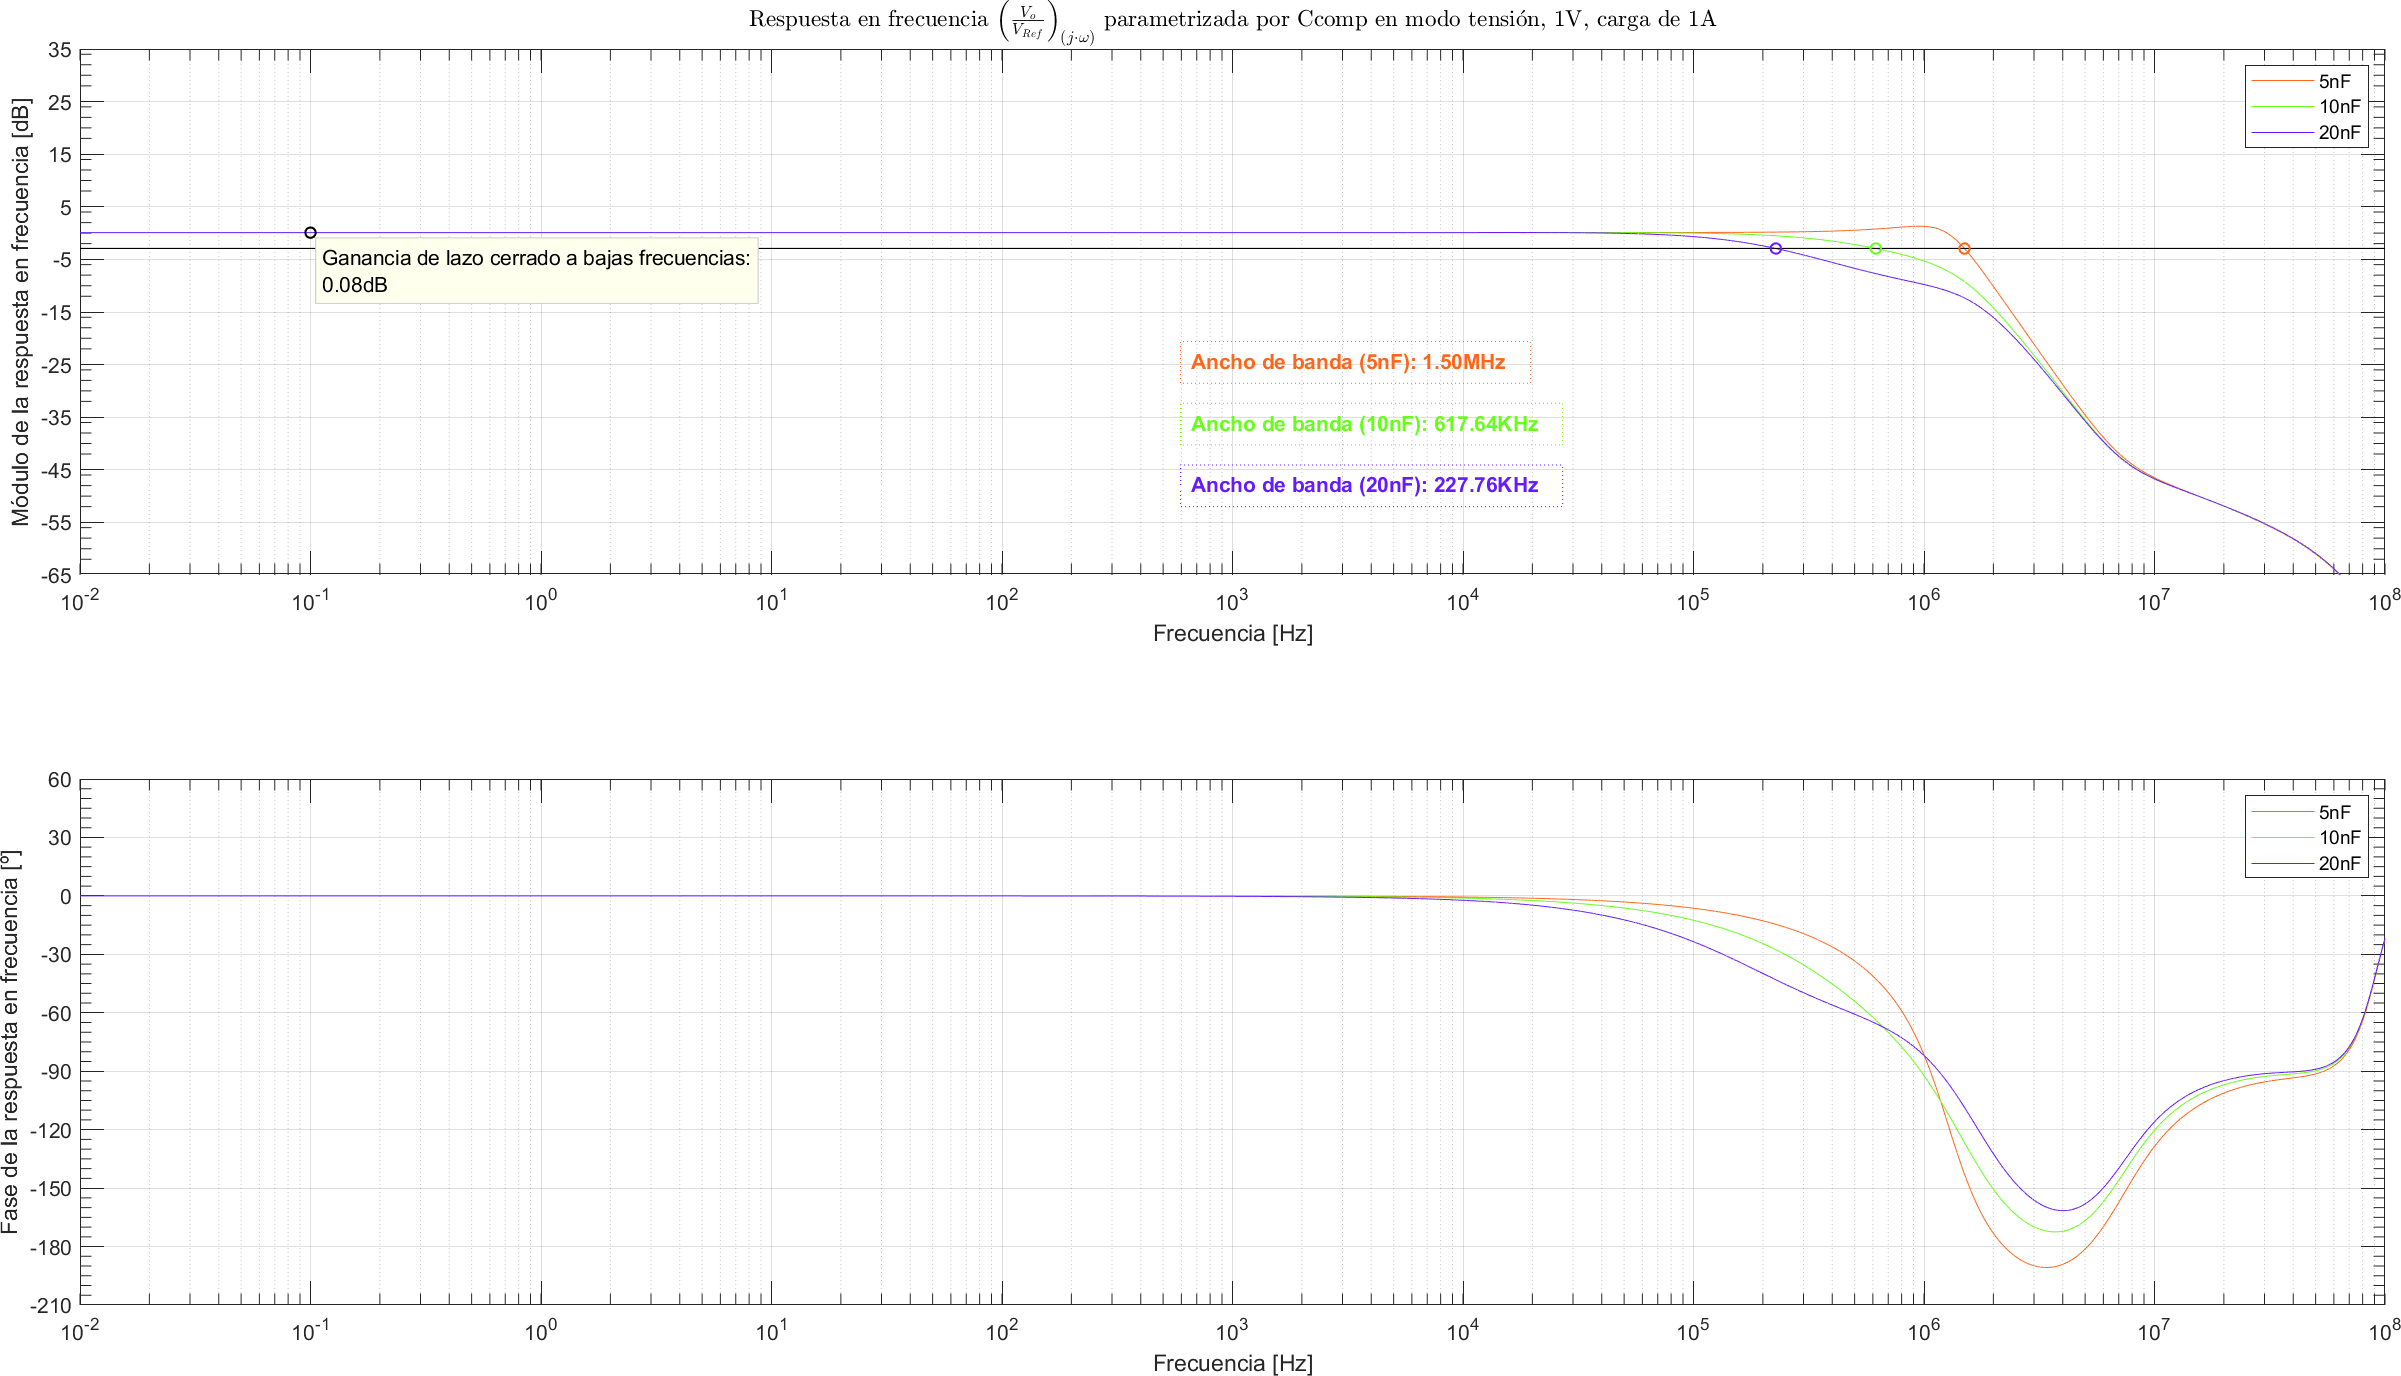
\includegraphics[width=1.1 \textwidth, angle=90]{./img/plots/rf/power_supply_CCOMP_RF_Modo2.png}
%\caption{\label{fig:fig_power_supply_CCOMP_RF_Modo2}\footnotesize{Respuesta en frecuencia en modo tensión, $V_{out} = 1 \si[per-mode=symbol]{\volt}$, en función de la frecuencia parametrizada por $C_{comp}$.}}
%\end{center}
%\end{figure}

